\documentclass[12pt]{article}
\usepackage{times}
\usepackage{geometry}
\usepackage[english]{babel}
\usepackage[utf8]{inputenc}
\usepackage{fancyhdr}
\usepackage{graphicx}
\usepackage{titlesec}
\usepackage{biblatex}
\usepackage{minted}
\usepackage{xcolor} % to access the named colour LightGray
\definecolor{LightGray}{gray}{0.9}

\addbibresource{References.bib}


\setlength{\headheight}{15.2pt}
\setcounter{secnumdepth}{3}
\rfoot{Pg: \thepage}

\geometry{
   a4paper,
   left = 25mm,
   top = 20mm,
}
\begin{document}
\thispagestyle{empty}

\section*{}
 {\LARGE\makebox[\textwidth]{\textbf{KATHMANDU UNIVERSITY}}}

\centerline{Department of Computer Science and Engineering}
\centerline{Dhulikhel,Kavre}
\begin{figure}[h]
    \centerline{
\includegraphics[width=50.546mm,height=50.546mm]{KU_Logo.png}}
\end{figure}

\centerline{\textbf{A Lab Report}}
\centerline{on}
\centerline{\underline{\textbf{"Lab 2"}}}

\vspace*{12mm}

\centerline{\textbf{[Code No. : COMP 342]}}
\centerline{(For partial fulfillment of 3rd Year/ 1st Semester in Computer Science)}

\vspace*{20mm}

\centerline{\textbf{Submitted by}}
\centerline{\textbf{Aayush Pokharel (Roll No. 43)}}


\vspace*{26mm}


\centerline{\textbf{Submitted to}}
\centerline{\textbf{Dhiraj Shrestha}}
\centerline{\textbf{Dept of Computer Science and Engineering}}

\vspace*{20mm}

\centerline{\textbf{Submission Date: 18th December, 2022}}



\clearpage
\thispagestyle{empty}

\section*{Abstract}
The report is drafted to meet the prerequisites to partially fulfill the COMP 342 course offered by the
Department of Computer Science and Engineering at Kathmandu University. This project is designed
to expand the knowledge of OpenGL and implement of different Line Drawing Algorithm that we learned in class.
\\\\
\textbf{Keywords:} OpenGL

\clearpage
\thispagestyle{empty}
\tableofcontents

\clearpage
\thispagestyle{empty}
\listoffigures

\clearpage
\pagenumbering{arabic}
\section{CHAPTER 1: INTRODUCTION}

\subsection{Environment}
The lab progam was written using the python programming language and OpenGL rendering Library. To write the program a virtual environment is
created and set of libraries is downloaded for the local virtual environment. Then the python interperter runs under this virtual environment
to run the program

\subsection{OpenGL}
The OpenGL rendering library is written in C programming language and a wrapper library called PyOpenGL is available under BSD-style Open-Source licence which translates the
API calls of OpenGL to Python programming. For this Lab, instead of the programmable shader pipeline of OpenGL, immedate pipeline (old pipeline) is used as it is easir to implement and doesn't
requre complex mathematics of calculating the buffer sizes, VBAs and VBOs.

\subsection{PyGame}
The PyGame is a cross-platform set of Python modules for game development. Despite being a complete package that can handle all the rendering in a highly abstracted manner, the
limitation of only using OpenGL for the lab work required that it only be used as windowing library under a double buffer system and all the relevant rendering process be done by PyOpenGL itself.

\section{CHAPTER 2: ALGORITHM}
We have read about three different Line Drawing Algorithms in our class. They are as folows:
\begin{itemize}
    \item Digital Differential Analyzer
    \item Bresenham
    \item MidPoint
\end{itemize}
\clearpage
\section{CHAPTER 3: CODE}

\subsection{Digital Differential Analyzer LDA}
This is the code for the Digital Differential Analyzer Algorithm.
\begin{minted}[
    frame=lines,
    framesep=2mm,
    baselinestretch=1.2,
    bgcolor=LightGray,
    fontsize=\footnotesize,
    linenos
    ]{python}
from typing import Tuple
import pygame as pg
from pygame import display, event
from pygame.locals import *

from OpenGL.GL import *
from OpenGL.GLU import *

# function of DDA
def DDA(start_coordinate: Tuple[int, int],
        end_coordinate: Tuple[int, int]):
    x1, y1 = start_coordinate
    x2, y2 = end_coordinate

    dx = abs(x2 - x1)
    dy = abs(y2 - y1)

    steps = max(dx, dy)

    Xinc = dx / steps
    Yinc = dy / steps

    X = x1
    Y = y1
    vertices: list[tuple[float, float]] = []
    for i in range(steps):
        vertices.append((X, Y))
        X = X + Xinc
        Y = Y + Yinc
    return vertices


def drawDDA():
    vertices = DDA((1, 1), (20, 40))
    glBegin(GL_LINE_STRIP)
    glColor3f(0.0, 0.0, 1.0)
    for v in vertices:
        x, y = v
        glVertex2f(x, y)
    glEnd()


def main():
    pg.init()
    display.set_mode((800, 800), DOUBLEBUF | OPENGL | GL_RGB)
    display.set_caption("DDA-Lab 2 | Aayush Pokharel")

    gluPerspective(200, 1, 1, 10)
    glTranslatef(0.0, 0.0, -10)

    while True:
        for ev in event.get():
            if ev.type == pg.QUIT:
                pg.quit()
                quit()

        drawDDA()
        display.flip()


if __name__ == "__main__":
    main()
\end{minted}

\subsection{Bresenham LDA}
This is the code for the Bresenham Line Drawing Algorithm.
\begin{minted}[
    frame=lines,
    framesep=2mm,
    baselinestretch=1.2,
    bgcolor=LightGray,
    fontsize=\footnotesize,
    linenos
    ]{python}
from typing import Tuple
import pygame as pg
from pygame import display, event
from pygame.locals import *

from OpenGL.GL import *
from OpenGL.GLU import *

# Creating a Type from Tuple
Coordinate = Tuple[int, int]

# function of BSA
def bresenham(startCoordinate: Coordinate, endCoordinate: Coordinate):
    x1, y1 = startCoordinate
    x2, y2 = endCoordinate

    m = abs((y2 - y1) / (x2 - x1))
    dx = abs(x2 - x1)
    dy = abs(y2 - y1)

    x, y = x1, y1

    coordinates: list[Coordinate] = []

    if m < 1:
        for i in range(0, dx):
            p = 2 * dy - dx
            x = x + 1
            if p < 0:
                coordinates.append((x, y))
                p = p + 2 * dy
            else:
                y = y + 1
                coordinates.append((x, y))
                p = p + 2 * (dy - dx)
    else:
        for i in range(0, dy):
            p = 2 * dx - dy
            y = y + 1
            if p < 0:
                coordinates.append((x, y))
                p = p + 2 * dx
            else:
                x = x + 1
                coordinates.append((x, y))
                p = p + 2 * (dx - dy)

    return coordinates


def NormalizeCoordinates(input, min, max):
    return (input - min) / (max - min)


def drawBSA():
    coordinates = bresenham((-1, -1), (2, 2))
    glBegin(GL_LINES)
    glColor3f(1.0, 0.0, 0.0)
    for v in coordinates:
        x, y = v
        print(v)
        glVertex2f(x, y)
    glEnd()


def main():
    pg.init()
    display.set_mode((800, 800), DOUBLEBUF | OPENGL | GL_RGB)
    display.set_caption("BSA-Lab 2 | Aayush Pokharel")

    gluPerspective(40, 1, 1, 10)
    glTranslatef(0.0, 0.0, -10)

    while True:
        for ev in event.get():
            if ev.type == pg.QUIT:
                pg.quit()
                quit()

        drawBSA()
        display.flip()


if __name__ == "__main__":
    main()

\end{minted}
\clearpage
\subsection{Midpoint LDA}
This is the code for the MidPoint Line Drawing Algorithm.
\begin{minted}[
    frame=lines,
    framesep=2mm,
    baselinestretch=1.2,
    bgcolor=LightGray,
    fontsize=\footnotesize,
    linenos
    ]{python}
from typing import Tuple
import pygame as pg
from pygame import display, event
from pygame.locals import *

from OpenGL.GL import *
from OpenGL.GLU import *

Coordinate = Tuple[int, int]


def midpoint(start_coordinate: Coordinate, end_coordinate: Coordinate):
    x1, y1 = start_coordinate
    x2, y2 = end_coordinate

    dx = abs(x2 - x1)
    dy = abs(y2 - y1)

    coordinates: list[Coordinate] = []

    if dy <= dx:
        d = dy - dx / 2
        x, y = x1, y1

        coordinates.append((x, y))

        while x < x2:
            x = x + 1

            if d < 0:
                d = d + dy
            else:
                d = d + dy - dx
                y = y + 1
            coordinates.append((x, y))
    elif dx <= dy:
        d = dx - dy / 2
        x, y = x1, y1

        coordinates.append((x, y))

        while y < y2:
            y = y + 1

            if d < 0:
                d = d + dx
            else:
                d = d + dx - dy
                x = x + 1
            coordinates.append((x, y))

    return coordinates


def drawMidPoint():
    vertices = midpoint((0, 0), (2, 2))
    glBegin(GL_LINES)
    glColor3f(0.0, 1.0, 0.0)
    for v in vertices:
        x, y = v
        glVertex2f(x, y)
    glEnd()


def main():
    pg.init()
    display.set_mode((800, 800), DOUBLEBUF | OPENGL | GL_RGB)
    display.set_caption("MidPoint-Lab 2 | Aayush Pokharel")

    gluPerspective(40, 1, 1, 10)
    glTranslatef(0.0, 0.0, -10)

    while True:
        for ev in event.get():
            if ev.type == pg.QUIT:
                pg.quit()
                quit()

        drawMidPoint()
        display.flip()


if __name__ == "__main__":
    main()

\end{minted}


\clearpage
\section{CHAPTER 3: SCREENSHOTS}
This is the screenshot of the executed program for DDA LDA.
\begin{figure}[h]
    \centerline{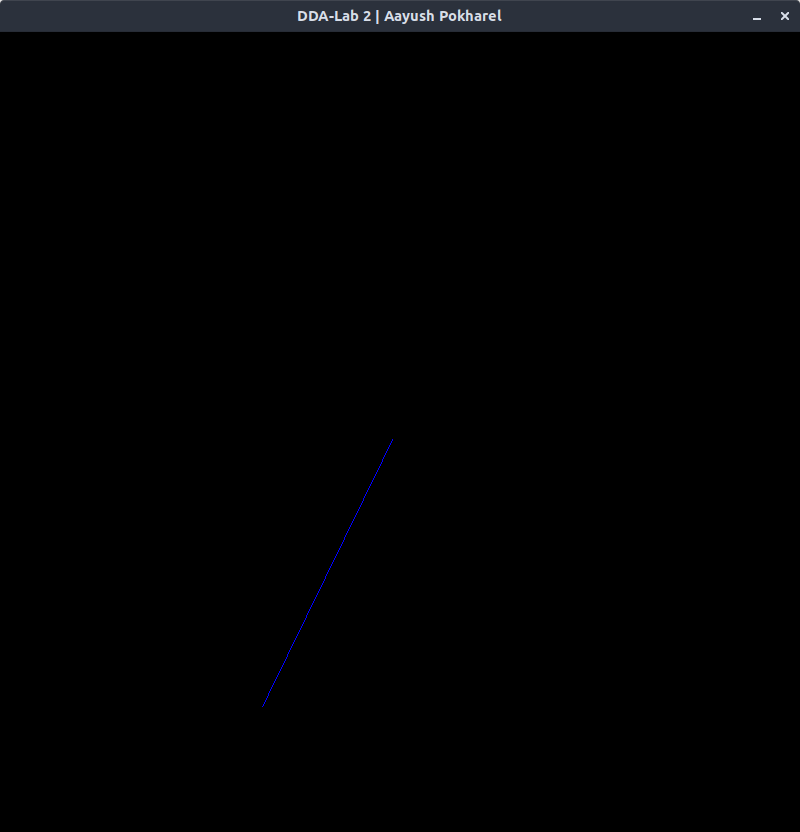
\includegraphics[height=100mm]{DDA.png}}
    \caption{Digital Differential Analyzer LDA}
    \label{fig}
\end{figure}
\clearpage
This is the screenshot of the executed program for DDA LDA.
\begin{figure}[h]
    \centerline{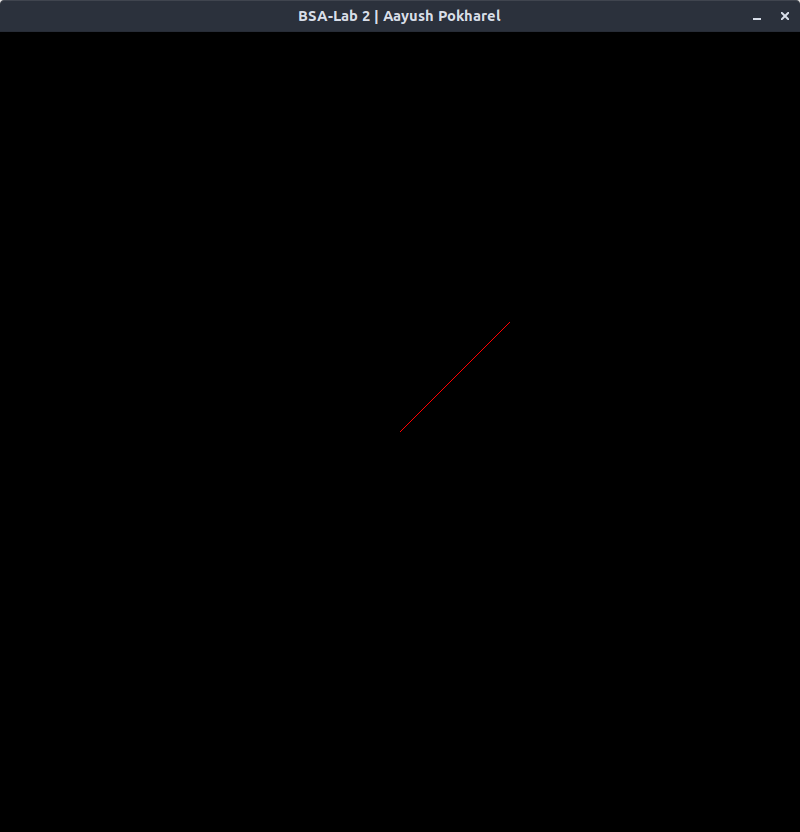
\includegraphics[height=100mm]{BSA.png}}
    \caption{Bresenham LDA}
    \label{fig}
\end{figure}
\clearpage
This is the screenshot of the executed program for MidPoint LDA.
\begin{figure}[h]
    \centerline{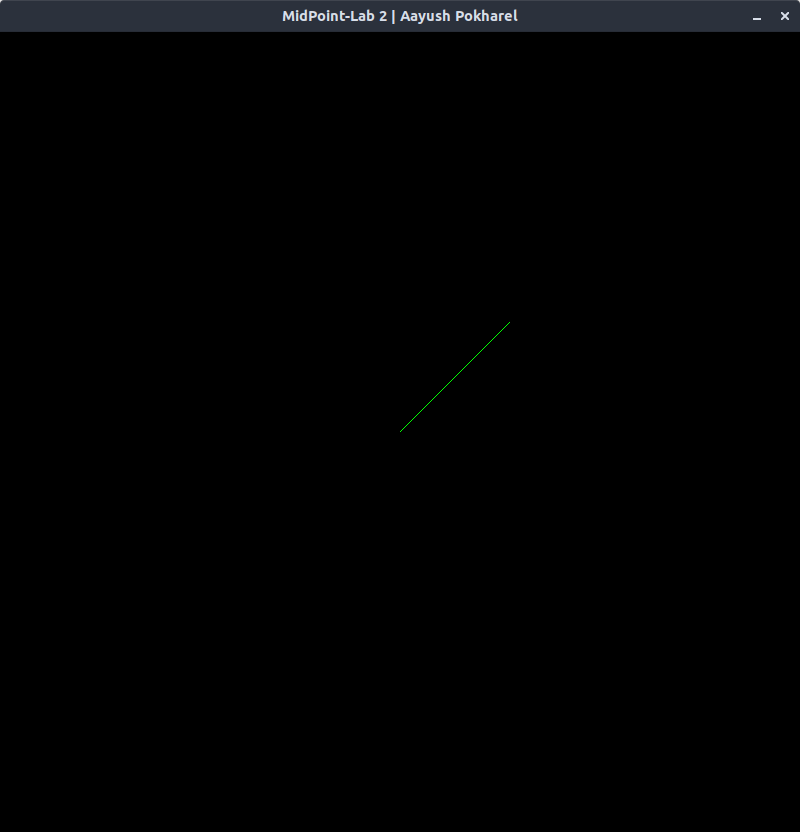
\includegraphics[height=100mm]{MidPoint.png}}
    \caption{MidPoint LDA}
    \label{fig}
\end{figure}

\section{CHAPTER 4: CONCLUSION}
In the nutshell, the lab was implement using the immedate rendering pipeline of OpenGL. Initially the same programmable shader pipeline was used but there
difficulty in implement the vertices to the buffer and had to be discarded. This lab uses the 2d rendering and to facilitate it the camera position was ket at a
fixed angle and a 2d vector was used. This 2d vector was implemented using python's typing library.
\clearpage
\thispagestyle{empty}
\printbibliography

\end{document}